\documentclass[addpoints]{exam}

%These tell TeX which packages to use.
\usepackage{array,epsfig}
\usepackage{amsmath}
\usepackage{amsfonts}
\usepackage{amssymb}
\usepackage{amsxtra}
\usepackage{amsthm}
\usepackage{mlextra} % must be below ams packages
\usepackage{mathrsfs}
\usepackage{color}
\usepackage{array}
\usepackage{graphicx}
\graphicspath{ {../art/} }
\usepackage{bm}
\usepackage{tikz}
\usepackage{multicol}

%Pagination stuff.
\setlength{\topmargin}{-.3 in}
\setlength{\oddsidemargin}{0in}
\setlength{\evensidemargin}{0in}
\setlength{\textheight}{9.in}
\setlength{\textwidth}{6.5in}



\newcommand{\twonode}{%
  \begingroup\normalfont
  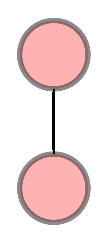
\includegraphics[height=\fontcharht\font`\b]{2nodetree.eps}%
  \endgroup
}


\begin{document}


\noindent
%\begin{tabular*}{\textwidth}{l @{\extracolsep{\fill}} r @{\extracolsep{6pt}} l}
%	{\large CS3920: Foundations of Computer Science} &  \makebox[3in]{\large Name:\enspace\hrulefill}\\
	%{Points: /\numpoints\. } \\
	%{\large June 8, 2018} & \\
%	{\large Quiz 2} & \\
%	{\large Points: \hspace{1cm}/\numpoints} & 
%\end{tabular*}\\

%\fbox{\fbox{\parbox{6in}{\textbf{Instructions}: Please answer the questions 
%			below to the best of your ability. Be sure to show your work where appropriate. 
%			This quiz is closed book, closed notes, closed computer.}}}\\
\begin{questions}
\question $F=(\lnot (P \lor Q) \iff (P \implies (Q \land \top))$. Draw the tree structure of $F$.

\vspace{30mm}

\question $F=(\lnot P \land \lnot Q) \implies (\lnot P \lor (Q \land R))$. Find the CNF of $F$, then write it in clausal form. 
Is F valid, satisfiable, falsifiable, or unsatisfiable?
\vspace{30mm}


\question $F=(P \lor Q) \implies (\lnot P \lor  R)$. Find the CNF of $F$, then write it in clausal form. 
Is F valid, satisfiable, falsifiable, or unsatisfiable?

\end{questions}
\end{document}


